\subsection{Generación de señalamiento paso a paso}

	Al ejecutar el RNA, primero detectará todos los \textit{netElements}, sus coordenadas iniciales y finales en la topología, y el sentido en el que fueron definidas. El resultado obtenido se muestra en el Cóodigo \ref{lst:EJ7_1}.
	
	\begin{lstlisting}[language = {}, caption = Detección de \textit{netElements} por parte del RNA , label = {lst:EJ7_1}]
	###### Starting Railway Network Analyzer #####
	Reading .railML file
	Creating railML object
	Analyzing railML object
	Analyzing graph
	ne1 [-770, -30] [260, -30] >>
	ne31 [554, 480] [1190, 480] >>
	ne32 [554, 480] [1460, 957] >>
	ne40 [260, -30] [554, 480] >>
	ne41 [260, -30] [1040, -420] >>
	ne42 [1040, -420] [1730, -420] >>
	ne43 [1040, -420] [440, -420] <<
	The network is connected
	\end{lstlisting}
	
	Por ejemplo, el \textit{netElement} ne42 inicia en la coordenada (1040;-420) y finaliza en la coordenada (1730;-420). El símbolo $>>$ indica que ne1 se encuentra definido de izquierda a derecha, ya que la componente x de la coordenada final es mayor a la de la coordenada inicial, teniendo la misma componente y. Además, se puede comprobar que la lista obtenida en consistente con la Figura \ref{fig:EJ7_2}. Por ejemplo, ne1, ne40 y ne41 comparten la coordenada (260;-30), que coincide con la coordenada del cambio de vías Sw18.
	
	A continuación, el RNA detectará la infraestructura ferroviaria, las curvas peligrosas y los puntos medios de los netElements que el RNA considera demasiado largos. El resultado de este proceso se puede visualizar en el Código \ref{lst:EJ7_2} y puede leerse también en el archivo Infrastructure.RNA.
	
	\begin{lstlisting}[language = {}, caption = Detección de puntos críticos por parte del RNA , label = {lst:EJ1_2}]
	Analyzing infrastructure --> Infrastructure.RNA
	Detecting Danger --> Safe_points.RNA
	ne1 has a Middle point @ [-564.0, -30]
	ne1 has a Middle point @ [-358.0, -30]
	ne1 has a Middle point @ [-152.0, -30]
	ne1 has a Middle point @ [54.0, -30]
	ne31 has a Middle point @ [766.0, 480]
	ne31 has a Middle point @ [978.0, 480]
	ne32 has a Curve(2 lines) @ [[830, 957]]
	ne41 has a Curve(2 lines) @ [[650, -30]]
	ne42 has a Middle point @ [1270.0, -420]
	ne42 has a Middle point @ [1500.0, -420]
	ne43 has a Middle point @ [640.0, -420]
	ne43 has a Middle point @ [840.0, -420]
	\end{lstlisting}
	
	Una vez que el RNA detectó cada punto crítico de la red ferroviaria, procede a generar el señalamiento. El orden de generación no es importante, pero para poder describirlo de forma consistente se iniciará generando el señalamiento para proteger los finales de vías, las junturas entre rieles, las plataformas, los cruces de vía y los cambios de vías. Luego se procederá a mostrar el señalamiento pre y post simplificación. Las señales generadas para proteger los finales de vías relativos y absolutos son ilustradas en la Figura \ref{fig:EJ7_3}.
	
	\begin{figure}[H]
		\centering
		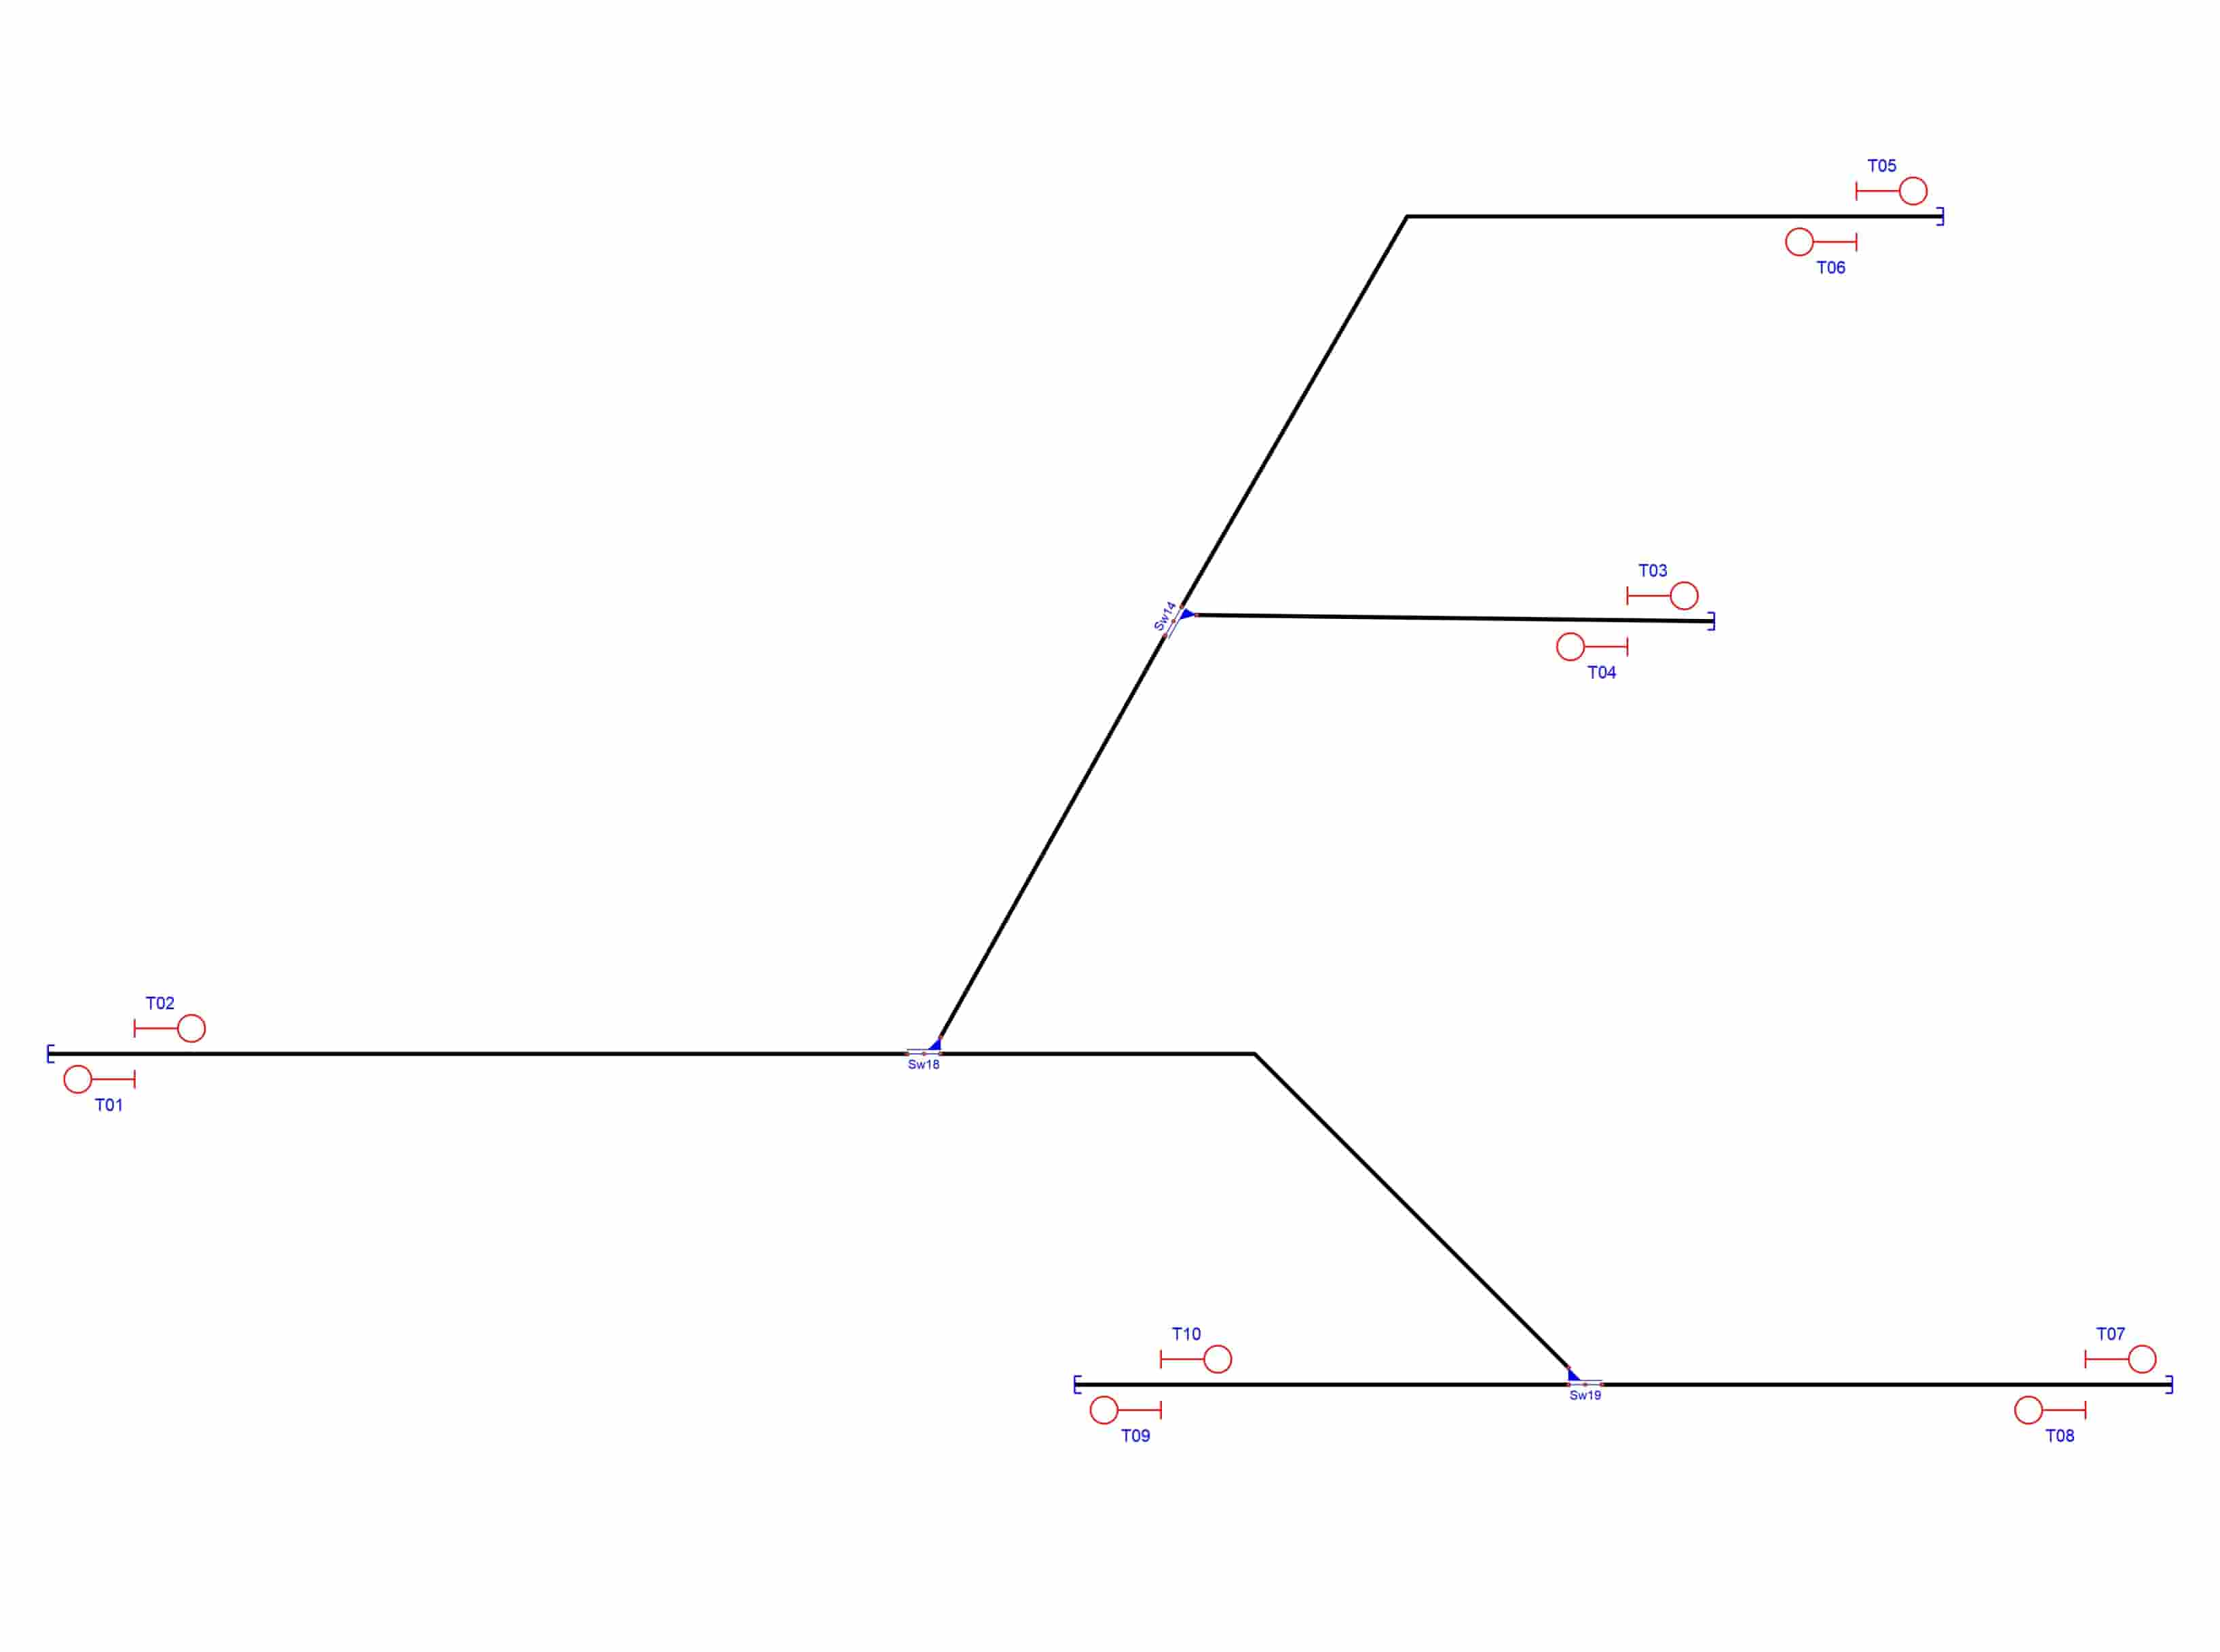
\includegraphics[width=1\textwidth]{resultados-obtenidos/ejemplo7/images/7_step1.png}
		\centering\caption{Señalamiento generado por el RNA para proteger el fin de vía.}
		\label{fig:EJ7_3}
	\end{figure}
	
	Los finales de vías absolutos son protegidos por las señales de parada T01, T03, T05, T07 y T09; y las señales de partida son T02, T04, T06, T08 y T10. No existen finales de vías relativos que proteger, por lo que el RNA asigno señalamiento para ese fin. Al tampoco existir junturas que proteger, la Figura \ref{fig:E71_4} no presenta cambios.
	
	\begin{figure}[H]
		\centering
		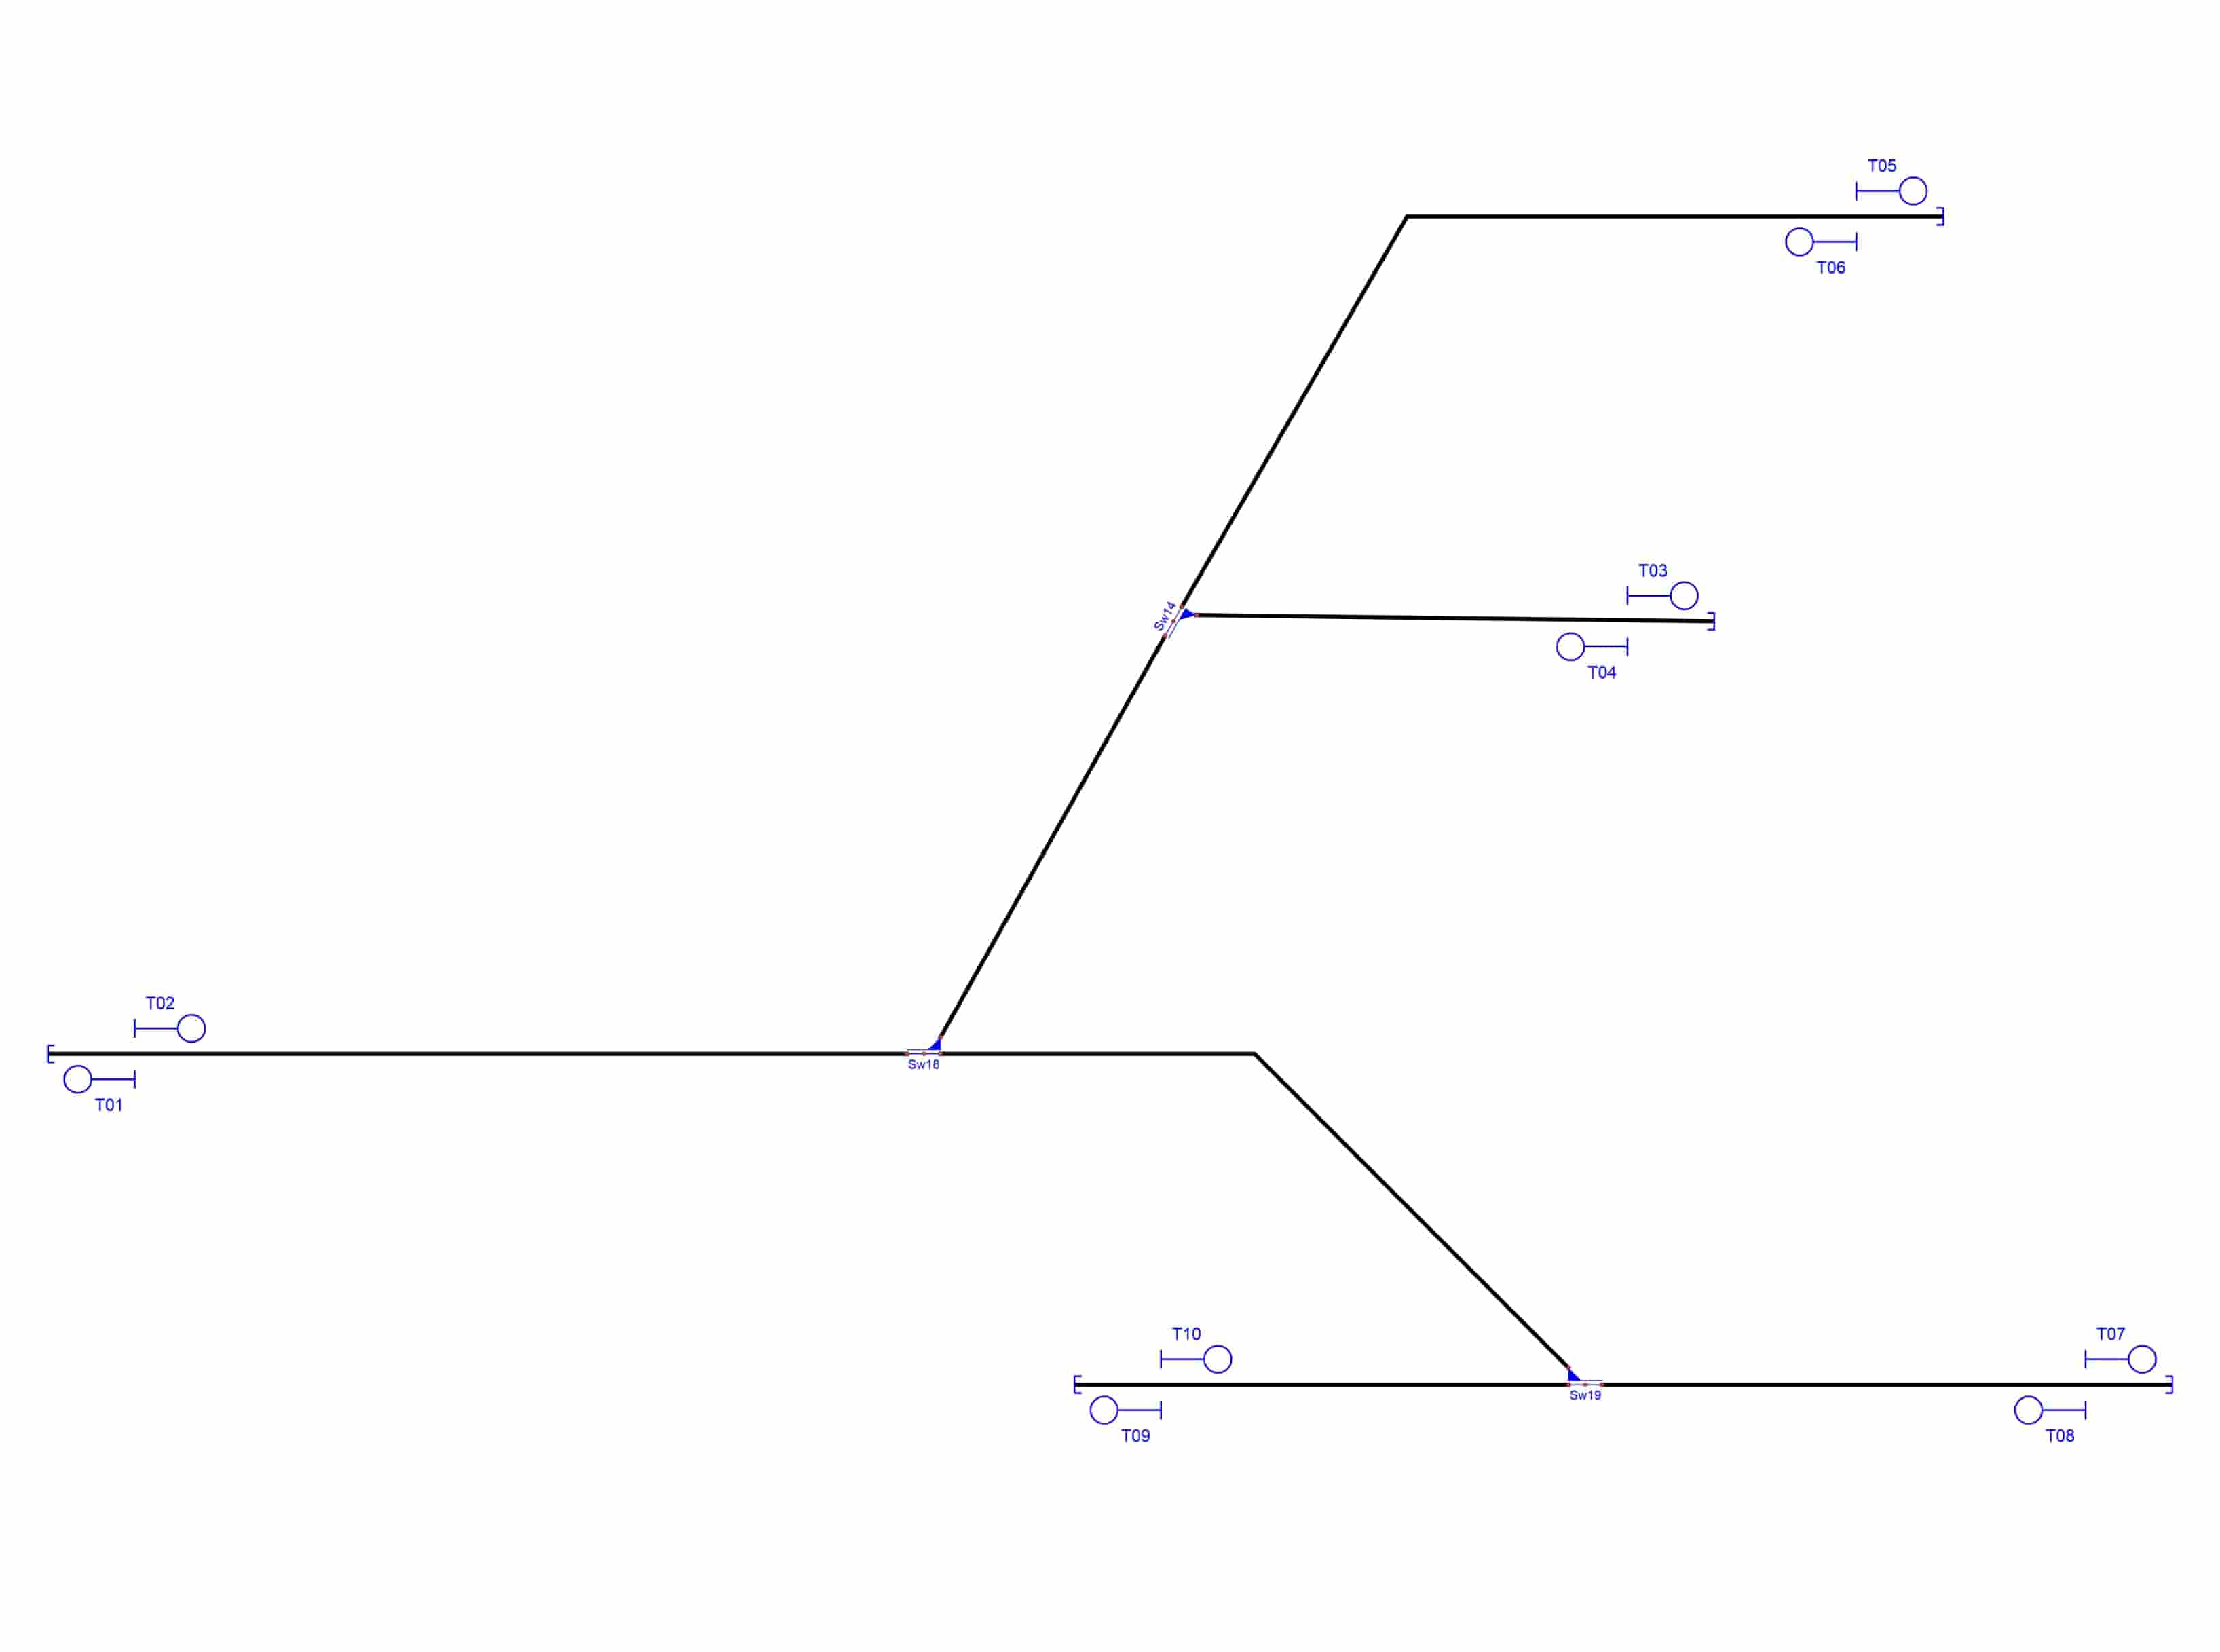
\includegraphics[width=1\textwidth]{resultados-obtenidos/ejemplo7/images/7_step2.png}
		\centering\caption{Señalamiento generado por el RNA para proteger las junturas.}
		\label{fig:EJ7_4}
	\end{figure}
	
	Al generar el señalamiento para proteger la infraestructura, tal como se explicó en la Sección \ref{sec:horizontal}, el Algoritmo \ref{alg:horizontal} simplificará las señales entre dos elementos ferroviarios si no existe espacio suficiente entre ellos. Al no existir plataformas o cruces de vías el señalamiento que se ilustra en la Figura \ref{fig:EJ7_5} no presenta cambios.
	
	\begin{figure}[H]
		\centering
		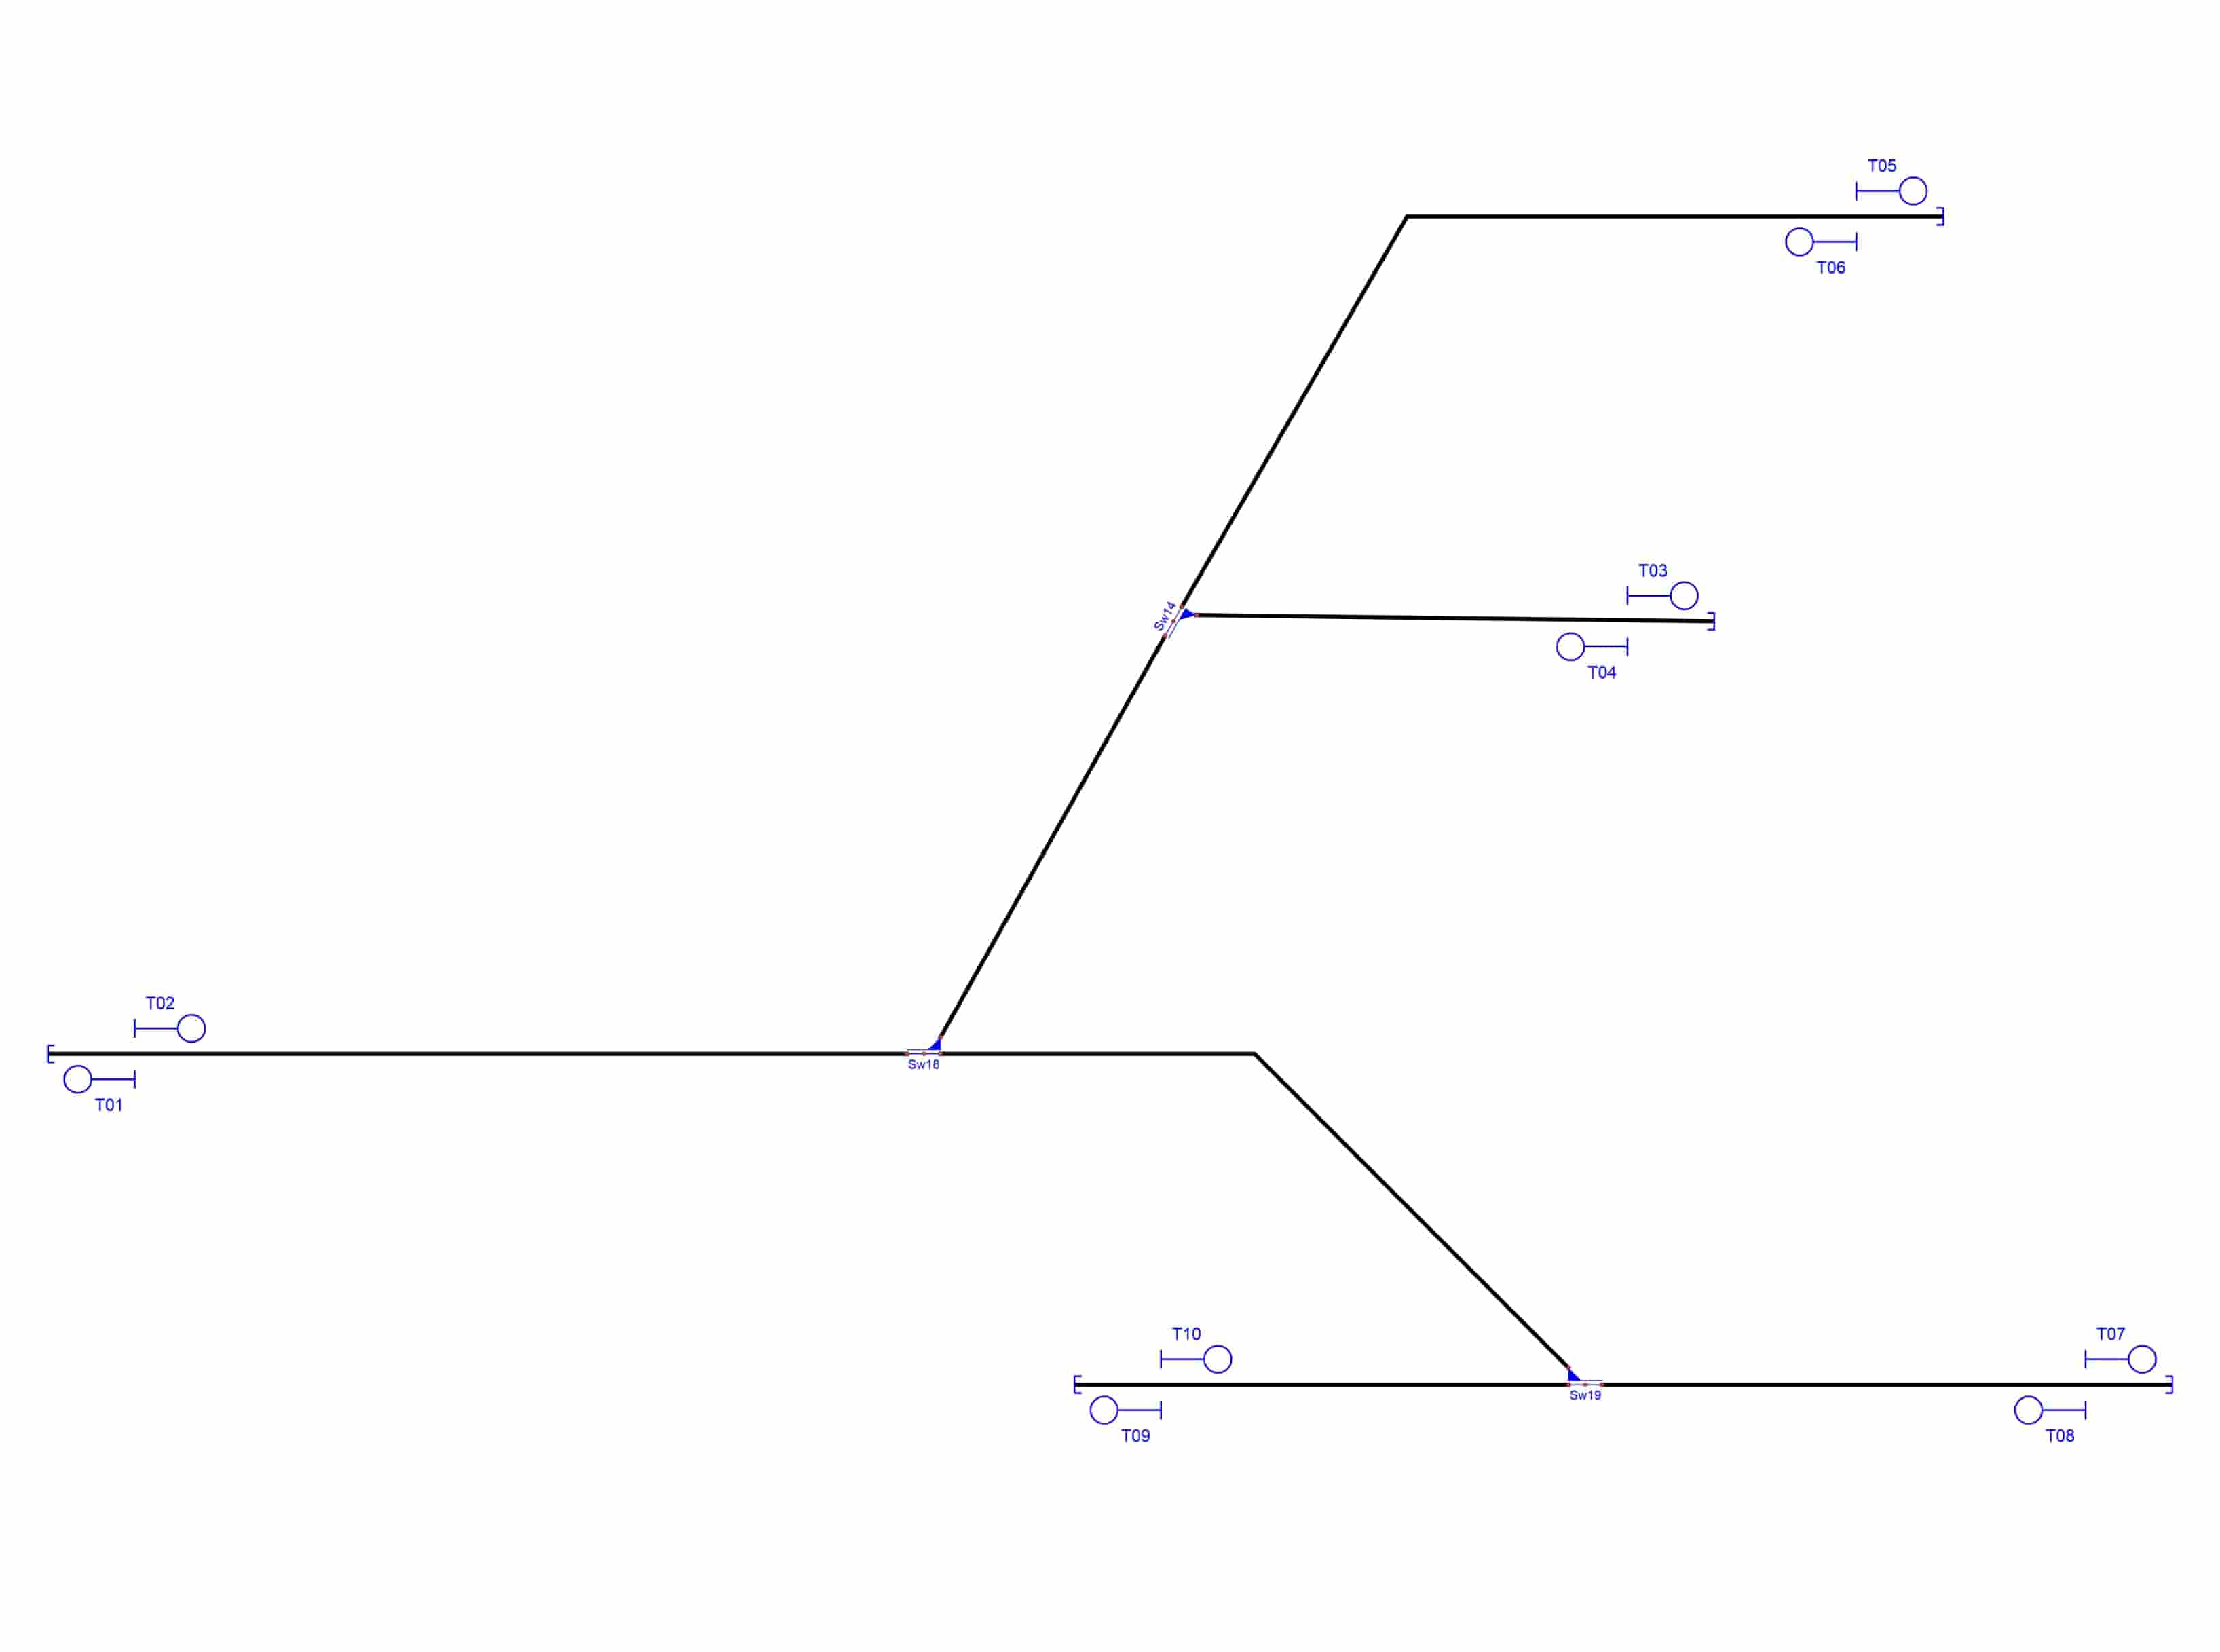
\includegraphics[width=1\textwidth]{resultados-obtenidos/ejemplo7/images/7_step3.png}
		\centering\caption{Señalamiento generado por el RNA para proteger plataformas y cruces de vía.}
		\label{fig:EJ7_5}
	\end{figure}
	
	El RNA generó las señales S14, C13 y H15 para proteger el cambio de vías Sw18; las señales C11, B12 y H16 para proteger el cambio de vías Sw14 y las señales S19, C17, B18 y H20 para proteger el cambio de vías Sw19. Las señales mencionadas se encuentran resaltadas en rojo en la Figura \ref{fig:EJ7_6}.
	
	\begin{figure}[H]
		\centering
		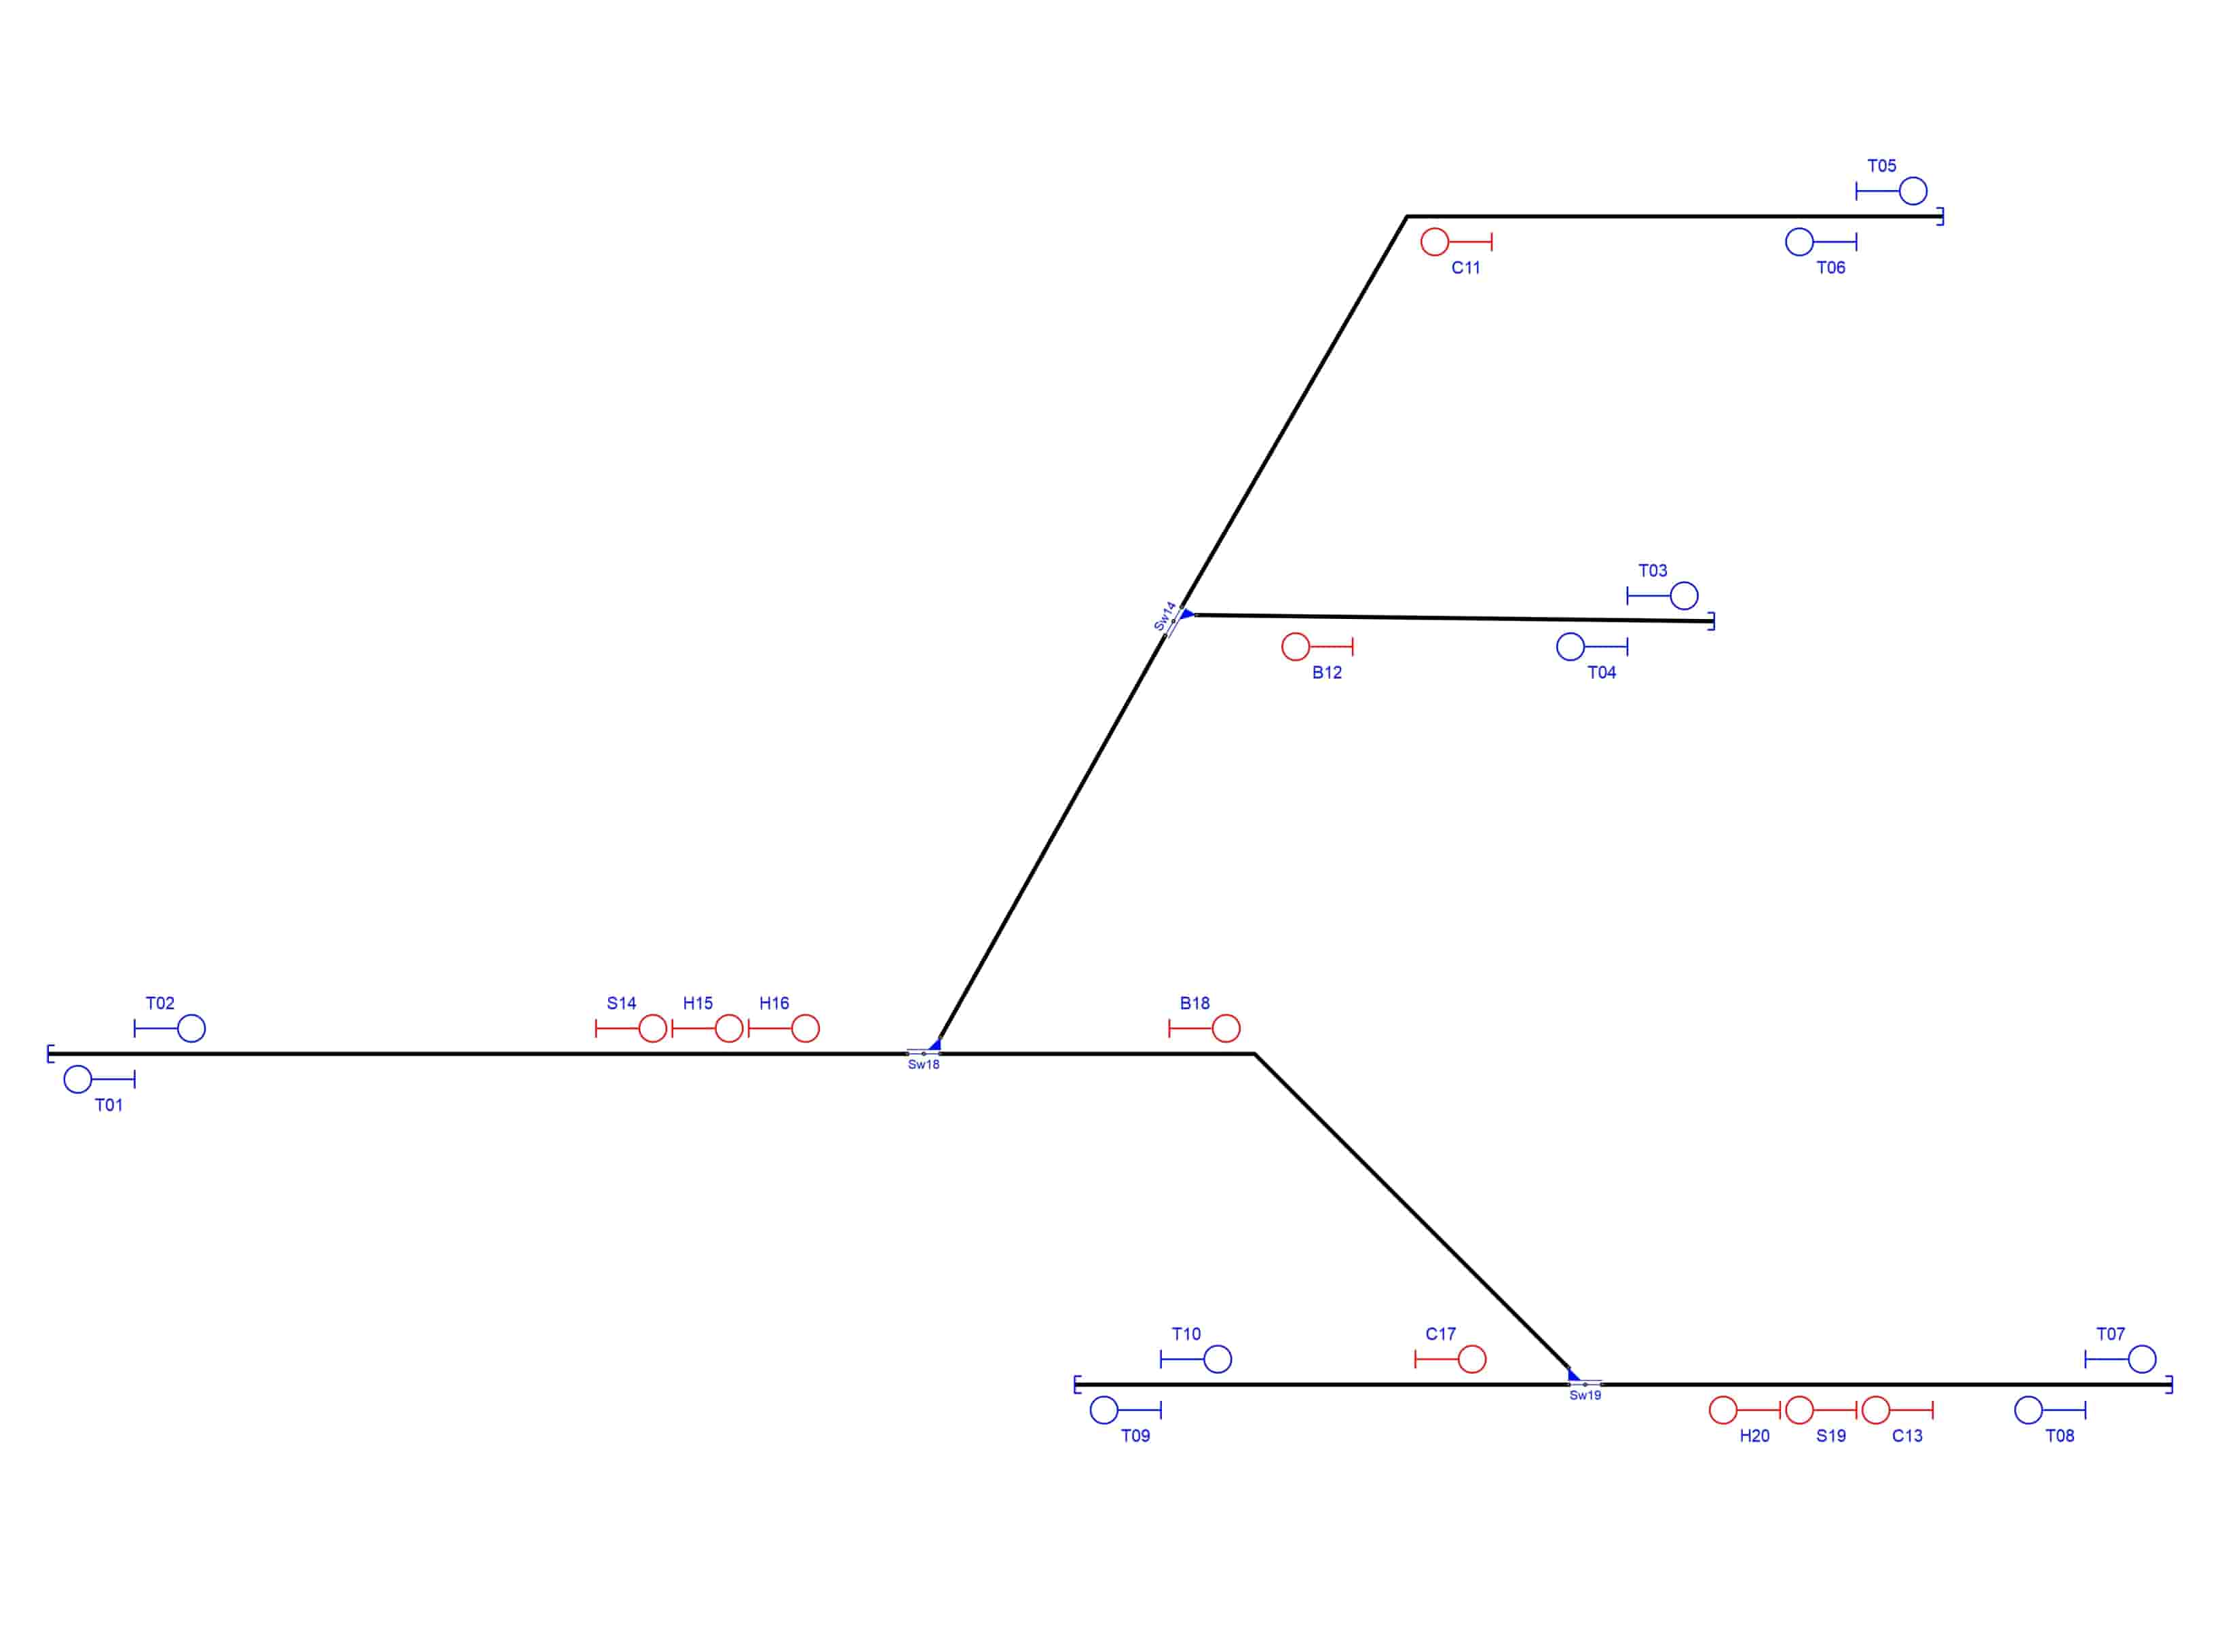
\includegraphics[width=1\textwidth]{resultados-obtenidos/ejemplo7/images/7_step4.png}
		\centering\caption{Señalamiento generado por el RNA para proteger los cambios de vías.}
		\label{fig:EJ7_6}
	\end{figure}
	
	Una vez obtenido todo el señalamiento, el RNA procede a simplificar las señales redundantes, repetidas o cuyas funciones o ubicaciones se superponen entre sí. El proceso de simplificación de señales fue explicado en la Sección \label{sec:simplificacion}. El Algoritmo \ref{alg:vertical} de herencia vertical fue aplicado en las señales B entre los cambios de vías Sw18 y Sw19, desplazando las señales hasta convertirlas en las señales B12 y B18 respectivamente. Análogamente, las señales C y S del \textit{netElement} se convirtieron en las señales H15 y C17 respectivamente.
	
	Las señales simplificadas al aplicar el Algoritmo \ref{alg:horizontal} de herencia horizontal son: C11, B12, H15, H16, C17, C13, S19 y H20. Las señales H15 y H16 fueron eliminadas por su cercanía con la señal S14, con la cual comparten dirección y sentido. Lo mismo ocurre entre las señales H20 y C13. En todos los casos, se aplicó el Algoritmo \ref{alg:horizontal}, diseñado para agrupar objetos cercanos como un único objeto, generando el señalamiento acorde a los elementos contenidos en cada extremo del nuevo elemento contenedor.
	
	Finalmente, las señales son simplificadas aplicando el Algoritmo \ref{alg:reduction} de eliminación por prioridad de señales. El resultado de este proceso es detallado en el Código \ref{lst:EJ7_3}.
	
	\begin{lstlisting}[language = {}, caption = Reducción de señalamiento por prioridad de señales, label = {lst:EJ7_3}]
	Reducing redundant signals
	T priority removing sig12 for sig04
	T priority removing sig11 for sig06
	T priority removing sig13 for sig08
	T priority removing sig19 for sig08
	T priority removing sig17 for sig10
	Same position removing sig15 for sig14
	Same position removing sig16 for sig14
	Same position removing sig20 for sig13
	\end{lstlisting}
	
	El resultado de la simplificación del señalamiento se ilustra en la Figura \ref{fig:EJ7_7}.
	
	\begin{figure}[H]
		\centering
		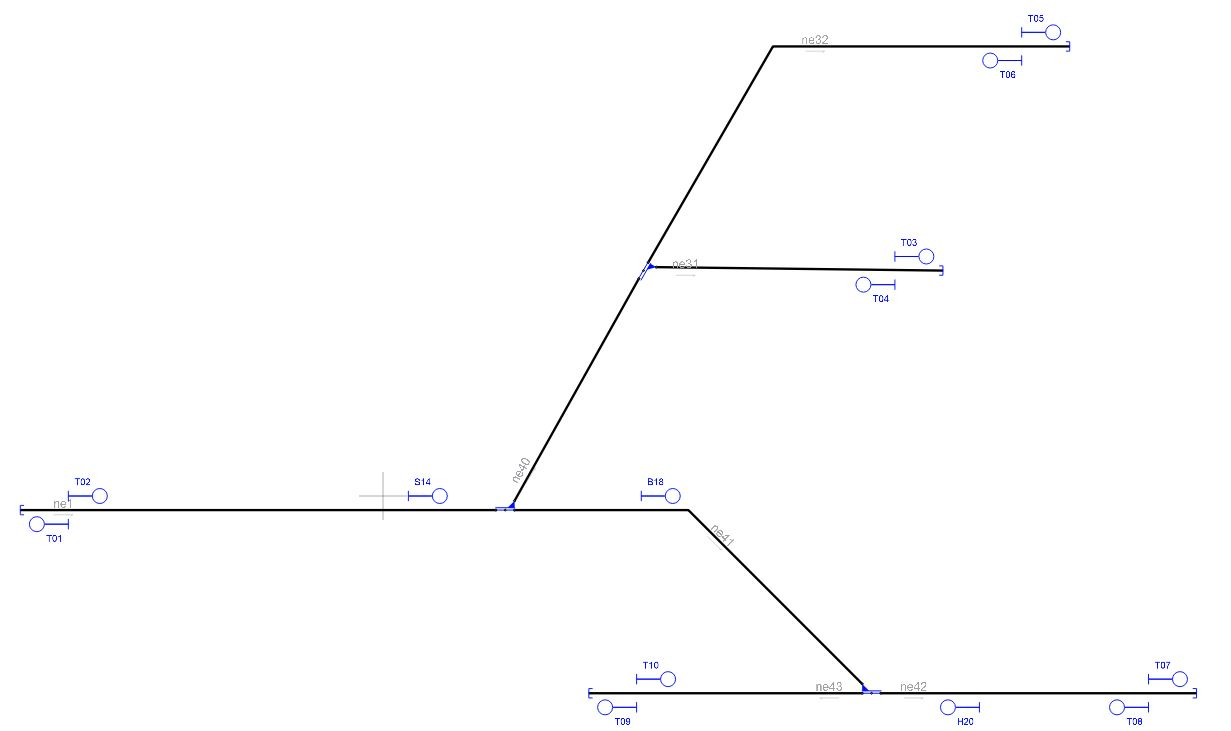
\includegraphics[width=1\textwidth]{resultados-obtenidos/ejemplo7/images/7_RNA.png}
		\centering\caption{Señalamiento generado y simplificado por el RNA.}
		\label{fig:EJ7_7}
	\end{figure}
	
	Al finalizar la generación del señalamiento, el RNA debe detectar todas las posibles rutas admitidas por la red para crear la tabla de enclavamientos. El RNA exporta los resultados del análisis en los siguientes cuatro documentos:
	
	Infrastructure.RNA (Código \ref{lst:EJ1_4}): resumen de cada elemento ferroviario en cada \textit{netElement}.
	
	\begin{lstlisting}[language = {}, caption = Infrastructure.RNA, label = {lst:EJ1_4}]
	Nodes: 7|Switches: 3|Signals: 0|Detectors: 0|Ends: 5|Barriers: 0
	Node ne1:
		Track = track1
		Type = BufferStop -> ['bus1']
		Neighbours = 2 -> ['ne41', 'ne40']
		Switches -> Sw18
			ContinueCourse -> right -> ne41
			BranchCourse -> left -> ne40
	Node ne31:
		Track = track2
		Type = BufferStop -> ['bus4']
		Neighbours = 2 -> ['ne40', 'ne32']
	Node ne32:
		Track = track4
		Type = BufferStop -> ['bus35']
		Neighbours = 2 -> ['ne31', 'ne40']
	Node ne40:
		Track = track3
		Neighbours = 4 -> ['ne1', 'ne31', 'ne32', 'ne41']
		Switches -> Sw14
			ContinueCourse -> left -> ne32
			BranchCourse -> right -> ne31
	Node ne41:
		Track = track5
		Neighbours = 4 -> ['ne1', 'ne40', 'ne42', 'ne43']
	Node ne42:
		Track = track6
		Type = BufferStop -> ['bus48']
		Neighbours = 2 -> ['ne41', 'ne43']
		Switches -> Sw19
			ContinueCourse -> left -> ne43
			BranchCourse -> right -> ne41
	Node ne43:
		Track = track7
		Type = BufferStop -> ['bus47']
		Neighbours = 2 -> ['ne41', 'ne42']
	\end{lstlisting}
	
	SafePoints.RNA (Código \ref{lst:EJ7_5}): coordenadas absolutas de cada punto donde puede colocarse una señal, en cada \textit{netElement}.
	
	\begin{lstlisting}[language = {}, caption = SafePoints.RNA, label = {lst:EJ7_5}]
	ne1:
		Next: [[-564.0, -30], [-358.0, -30], [-152.0, -30], [54.0, -30]]
		Prev: [[-564.0, -30], [-358.0, -30], [-152.0, -30], [54.0, -30]]
	ne31:
		Next: [[766.0, 480], [978.0, 480]]
		Prev: [[766.0, 480], [978.0, 480]]
	ne32:
		Prev: [[930.0, 957]]
	ne41:
		Next: [[550.0, -30]]
	ne42:
		Next: [[1270.0, -420], [1500.0, -420]]
		Prev: [[1270.0, -420], [1500.0, -420]]
	ne43:
		Next: [[640.0, -420], [840.0, -420]]
		Prev: [[640.0, -420], [840.0, -420]]
	\end{lstlisting}
	
	Signalling.RNA (Código \ref{lst:EJ7_6}): información detallada de todas las señales generadas.
	
	\begin{lstlisting}[language = {}, caption = Signalling.RNA, label = {lst:EJ7_6}]
	sig01 [T01] <<:
		From: ne1 | To: bus1_left
		Type: Stop | Direction: reverse | AtTrack: right 
		Position: [-670, 30] | Coordinate: 0.0970
	sig02 [T02] >>:
		From: ne1 | To: ne1_right
		Type: Stop | Direction: normal | AtTrack: left 
		Position: [-670, 30] | Coordinate: 0.0970
	sig03 [T03] >>:
		From: ne31 | To: bus4_right
		Type: Stop | Direction: normal | AtTrack: left 
		Position: [1090, -480] | Coordinate: 0.8427
	sig04 [T04] <<:
		From: ne31 | To: ne31_left
		Type: Stop | Direction: reverse | AtTrack: right 
		Position: [1090, -480] | Coordinate: 0.8427
	sig05 [T05] >>:
		From: ne32 | To: bus35_right
		Type: Stop | Direction: normal | AtTrack: left 
		Position: [1360, -957] | Coordinate: 0.9153
	sig06 [T06] <<:
		From: ne32 | To: ne32_left
		Type: Stop | Direction: reverse | AtTrack: right 
		Position: [1360, -957] | Coordinate: 0.9153
	sig07 [T07] >>:
		From: ne42 | To: bus48_right
		Type: Stop | Direction: normal | AtTrack: left 
		Position: [1630, 420] | Coordinate: 0.8550
	sig08 [T08] <<:
		From: ne42 | To: ne42_left
		Type: Stop | Direction: reverse | AtTrack: right 
		Position: [1630, 420] | Coordinate: 0.8550
	sig09 [T09] <<:
		From: ne43 | To: bus47_left
		Type: Stop | Direction: normal | AtTrack: left 
		Position: [540, 420] | Coordinate: 0.1666
	sig10 [T10] >>:
		From: ne43 | To: ne43_right
		Type: Stop | Direction: reverse | AtTrack: right 
		Position: [540, 420] | Coordinate: 0.1666
	sig14 [S14] >>:
		From: ne1 | To: ne1_right
		Type: Circulation | Direction: normal | AtTrack: left 
		Position: [54.0, 30] | Coordinate: 0.8
	sig18 [B18] >>:
		From: ne41 | To: ne41_right
		Type: Manouver | Direction: normal | AtTrack: left 
		Position: [550.0, 30] | Coordinate: 0.8937
	sig20 [H20] <<:
		From: ne42 | To: ne42_left
		Type: Manouver | Direction: reverse | AtTrack: right 
		Position: [1270.0, 420] | Coordinate: 0.3333
	\end{lstlisting}
	
	Routes.RNA (Código \ref{lst:EJ7_7}): tabla de enclavamientos.
	
	\begin{lstlisting}[language = {}, caption = Routes.RNA, label = {lst:EJ7_7}]
	route_1 [sig02 >> sig14]:
		Path: ['ne1']
		Switches: ['Sw18']
	route_2 [sig04 << sig01]:
		Path: ['ne31', 'ne40', 'ne1']
		Switches: ['Sw14', 'Sw18']
	route_3 [sig06 << sig01]:
		Path: ['ne32', 'ne40', 'ne1']
		Switches: ['Sw14', 'Sw18']
	route_4 [sig08 << sig20]:
		Path: ['ne42']
		Switches: ['Sw19']
	route_5 [sig10 >> sig07]:
		Path: ['ne43', 'ne42']
		Switches: ['Sw19']
	route_6 [sig14 >> sig18]:
		Path: ['ne1', 'ne41']
		Switches: ['Sw18']
	route_7 [sig14 >> sig03]:
		Path: ['ne1', 'ne40', 'ne31']
		Switches: ['Sw14', 'Sw18']
	route_8 [sig14 >> sig05]:
		Path: ['ne1', 'ne40', 'ne32']
		Switches: ['Sw14', 'Sw18']
	route_9 [sig18 >> sig07]:
		Path: ['ne41', 'ne42']
		Switches: ['Sw19']
	route_10 [sig20 << sig01]:
		Path: ['ne42', 'ne41', 'ne1']
		Switches: ['Sw18', 'Sw19']
	route_11 [sig20 << sig09]:
		Path: ['ne42', 'ne43']
		Switches: ['Sw19']
	\end{lstlisting}